\section{Goal 1: anomaly and bias detection}
\label{sec:goal1}
\goalbadge{GOAL 1} The system must detect equipment faults, degraded sensors, and biased, corrupted or falsified readings, and distinguish a real grid event from a data-quality problem~\cite{brief}. The tested models and the curves of this report are all in this section.

\subsection{Architecture of Goal 1}
\begin{figure}[!h]
\centering
\begin{tikzpicture}
\node[gbox,text width=2.6cm] (w) at (1.6,0.6) {\textbf{15-minute window}\\past measurements of one house};
\node[gbox,text width=3.6cm] (b1) at (6.2,1.7) {\textbf{Physics checks}\\are the relations between voltage, current and power respected?};
\node[gbox,text width=3.6cm] (b2) at (6.2,-0.5) {\textbf{LightGBM model}\\is this behaviour normal for this house?};
\node[dbox,text width=3.0cm] (b3) at (6.2,-2.5) {\textbf{Feeder context}\\neighbours, upstream meter (experiment)};
\node[hbox,text width=2.7cm] (ca) at (10.7,0.6) {\textbf{Calibration and abstention}\\numerical confidence};
\node[gbox,text width=3.0cm] (v) at (14.4,0.6) {\textbf{Verdict}\\normal, measurement problem, real event, or unresolved};
\draw[arr] (w.east) -- ++(0.4,0) |- (b1.west); \draw[arr] (w.east) -- ++(0.4,0) |- (b2.west);
\draw[arr] (b1.east) -- ++(0.35,0) |- (ca.west); \draw[arr] (b2.east) -- ++(0.35,0) |- (ca.west);
\draw[darr] (b3.east) -- ++(0.35,0) |- (ca.west);
\draw[arr] (ca)--(v);
\end{tikzpicture}
\caption{Architecture of Goal~1. Detector v1 combines the physics checks and the model in one LightGBM model; the feeder context is a separate experiment.}
\end{figure}

\textbf{Principle.} A healthy meter respects a few physical relations (for example, apparent power equals voltage times current). A faulty sensor often breaks one of them; a real grid event respects them all, because the electrical state really changed. The detector therefore computes \emph{residuals} (the gaps to these relations), plus the length of frozen values, the share of missing data, variation statistics, and context (time of day, history from 60 minutes to 7 days). A check that cannot be evaluated is flagged, never counted as passed.

\subsection{Method and evaluation protocol}
\textbf{Detector v1.} A 15-minute window (stride 5), built only from past measurements, is classified by a LightGBM model~\cite{lightgbm} (three classes: normal, measurement problem, real event), then its confidence is calibrated by temperature scaling~\cite{guo}. A window raises an alert if its ``abnormal'' probability exceeds a threshold chosen on a validation slice; neighbouring alerts are merged into segments. We compare with five baselines: a robust $z$-score, Isolation Forest, One-Class SVM, a causal convolutional network (TCN) and an autoencoder.

\textbf{Protocol.} Per-window scores are inflated by correlated neighbouring windows, and ``point adjustment'' overstates detection~\cite{tatbul}. We therefore score \textbf{per event}: an alert matches an incident if it overlaps it within $\pm$15 minutes; we compute precision and recall per class, the \textbf{event macro-F1} (mean of the two fault classes) and \textbf{false alarms per day (FA/day)}. The split is by time (60\,\% training, 15\,\% calibration, 25\,\% test, with a 60-minute purge), and whole houses are held out.

\textbf{We audited our own benchmark.} The first injector modified channels that the loader computes from others without recomputing them: measurement faults produced impossible residuals, and a clue made it possible to guess the label (AUC 0.999). Injector v2 modifies only real registers; the AUC fell to 0.500 and permutation tests give chance level. The numbers went down (baseline window F1: 0.724 then 0.566; false alarms: 2.12 then 7.15 per day), but the conclusions are now defensible.

\subsection{Results on the corrected benchmark}
\begin{table}[!h]
\footnotesize\centering
\caption{Detector v1 against the baseline (LightGBM), per event. P/R = precision/recall. Synthetic faults on real data.}
\begin{tabularx}{\textwidth}{@{}llCCCC@{}}
\toprule
\hdr \textbf{Scenario} & \textbf{Model} & \textbf{Measurement P / R} & \textbf{Real event P / R} & \textbf{Macro-F1} & \textbf{FA/day}\\
\midrule
Training houses & baseline & 0.242 / 0.797 & 0.144 / 0.795 & 0.307 & 7.27\\
 & \textbf{v1} & 0.843 / 0.772 & 0.974 / 0.631 & \textbf{0.786} & 0.144\\
Held-out house 1 & baseline & 0.148 / 0.972 & 0.545 / 0.287 & 0.317 & 6.28\\
 & \textbf{v1} & 0.423 / 0.808 & 0.943 / 0.465 & \textbf{0.589} & 0.971\\
Held-out house 2 & baseline & 0.278 / 0.824 & 0.259 / 0.658 & 0.393 & 3.54\\
 & \textbf{v1} & 0.574 / 0.705 & 0.727 / 0.491 & \textbf{0.609} & 0.533\\
AMPds2 & baseline & 0.151 / 0.910 & 0.208 / 0.815 & 0.295 & 7.85\\
 & \textbf{v1} & 0.785 / 0.605 & 0.900 / 0.664 & \textbf{0.724} & 0.212\\
WPuQ (indicative) & \textbf{v1} & 0.882 / 0.827 & 0.667 / 0.690 & \textbf{0.766} & 0.253\\
\bottomrule
\end{tabularx}
\end{table}

\begin{figure}[!h]
\centering
\begin{tikzpicture}
\begin{axis}[ybar,bar width=6.5pt,width=8.0cm,height=3.7cm,ymin=0,ymax=1.0,
 symbolic x coords={inhouse,eco03,eco06,ampds,wpuq},xtick={inhouse,eco03,eco06,ampds,wpuq},
 xticklabels={Training,House 1,House 2,AMPds2,WPuQ},
 x tick label style={font=\sffamily\tiny},y tick label style={font=\sffamily\tiny},
 ylabel={event macro-F1},ylabel style={font=\sffamily\scriptsize},enlarge x limits=0.13,
 nodes near coords,every node near coord/.append style={font=\sffamily\tiny,rotate=90,anchor=west,/pgf/number format/.cd,fixed,precision=2},
 legend style={font=\sffamily\tiny,at={(0.5,1.03)},anchor=south,legend columns=2,draw=none}]
\addplot[fill=white,draw=black,pattern=north east lines] coordinates {(inhouse,0.307) (eco03,0.317) (eco06,0.393) (ampds,0.295)};
\addplot[fill=black!70,draw=black] coordinates {(inhouse,0.786) (eco03,0.589) (eco06,0.609) (ampds,0.724) (wpuq,0.766)};
\legend{Baseline,Detector v1}
\end{axis}
\begin{axis}[at={(8.6cm,0)},ybar,bar width=6.5pt,width=8.0cm,height=3.7cm,ymin=0,ymax=9.5,
 symbolic x coords={inhouse,eco03,eco06,ampds,wpuq},xtick={inhouse,eco03,eco06,ampds,wpuq},
 xticklabels={Training,House 1,House 2,AMPds2,WPuQ},
 x tick label style={font=\sffamily\tiny},y tick label style={font=\sffamily\tiny},
 ylabel={false alarms per day},ylabel style={font=\sffamily\scriptsize},enlarge x limits=0.13,
 nodes near coords,every node near coord/.append style={font=\sffamily\tiny,rotate=90,anchor=west,/pgf/number format/.cd,fixed,precision=2},
 legend style={font=\sffamily\tiny,at={(0.5,1.03)},anchor=south,legend columns=2,draw=none}]
\addplot[fill=white,draw=black,pattern=north east lines] coordinates {(inhouse,7.27) (eco03,6.28) (eco06,3.54) (ampds,7.85)};
\addplot[fill=black!70,draw=black] coordinates {(inhouse,0.144) (eco03,0.971) (eco06,0.533) (ampds,0.212) (wpuq,0.253)};
\legend{Baseline,Detector v1}
\end{axis}
\end{tikzpicture}
\caption{Event macro-F1 (left, higher is better) and false alarms per day (right, lower is better). WPuQ has no baseline and is indicative.}
\end{figure}

\textbf{The price of precision.} Detector v1 is an operating point that favours precision. Recall of three fault types collapses (\code{demand_step} 0.111; \code{duty_cycle} 0.086; \code{falsified} 0.029, against 0.63; 0.57; 0.23 before); the median delay rises from 2 to 10 minutes; in return, benign cases that raise an alarm drop from 66\,\% to 2\,\%. On unseen houses the F1 loses about 0.2. \code{falsified} respects every physical relation by construction: it is detected (0.743) but rarely classified correctly (0.343).

\begin{figure}[!h]
\centering
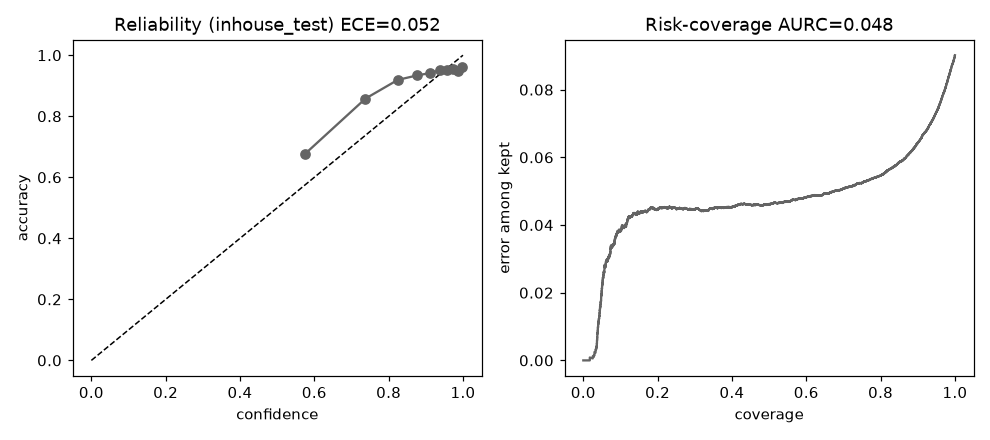
\includegraphics[width=0.5\textwidth]{figures/reliability.png}
\caption{Calibration of detector v1 on the training houses (calibration error 0.052): reliability diagram (left) and risk--coverage curve (right). Abstaining below 0.55 confidence cuts the baseline's false alarms from 7.15 to 1.92 per day, at the cost of lower recall (0.926 then 0.784).}
\end{figure}

\begin{table}[!h]
\small\centering
\caption{Baseline models on the training houses (window macro-F1; recall measurement / real event; p95 inference time per call on a laptop CPU, not a load test).}
\begin{tabularx}{\textwidth}{@{}lCCCCC@{}}
\toprule
\hdr \textbf{Model} & \textbf{Macro-F1} & \textbf{Recall} & \textbf{FA/day} & \textbf{Calib.} & \textbf{p95 (ms)}\\
\midrule
Robust $z$-score & 0.436 & 0.917 / 0.881 & 6.09 & 0.458 & 0.24\\
Isolation Forest & 0.432 & 0.946 / 0.938 & 8.45 & 0.223 & 14.30\\
One-Class SVM & 0.436 & 0.946 / 0.960 & 9.49 & 0.208 & 1.03\\
LightGBM & 0.566 & 0.934 / 0.926 & 7.15 & 0.076 & 1.79\\
Causal TCN (3 seeds) & 0.535 & 0.322 / 0.398 & 0.08 & 0.010 & 4.12\\
Convolutional autoencoder & -- & 0.174 / 0.040 & 0.05 & 0.012 & 0.74\\
\bottomrule
\end{tabularx}
\end{table}
LightGBM is the best baseline; the TCN is cautious and does not beat it. Without the physics residuals, the macro-F1 drops to 0.453. \textbf{Transfer from one dataset to another fails:} from ECO to AMPds2 without adaptation, LightGBM reaches 0.476 (0.613 on site); a per-house adaptation step is needed.

\textbf{Feeder context and fusion.} On a SimBench feeder, neighbouring and upstream meters add 4.1 points of event accuracy on the same feeder (95\,\% confidence interval 1.6 to 6.5) and 7.3 points on another feeder (4.9 to 9.9). Eight detectors reading the same meter are not eight confirmations: naive fusion becomes badly over-confident (confidence minus accuracy up to $+0.907$); fusion that accounts for provenance brings it back to $-0.017$ without improving accuracy. We report this negative result.

\textbf{Next steps (Phase 2).} Three extensions, each kept only if it beats a simpler model: \textbf{appliance-level consumption estimation} (NILM, causal TCN~\cite{seq2point}), \textbf{richer physics checks} (feeder balance, circuit model) and a \textbf{graph model} using relations between neighbouring houses.
